In 2017, Hurricane Maria hit Puerto Rico and produced extensive damage to buildings, homes, and roads, particularly along the east and southeast coast of the island. The storm resulted in loss of power to essentially all of the island's residents, the destruction of the majority of the island’s cellular communication networks, and damage to many highways and roads across the island, making it nearly impossible for emergency services ground vehicles to plan and navigate their routes. In the meantime, dozens of areas were isolated and without communication, and demand for medical care and supplies surged.

\begin{figure}[h]
    \centering
    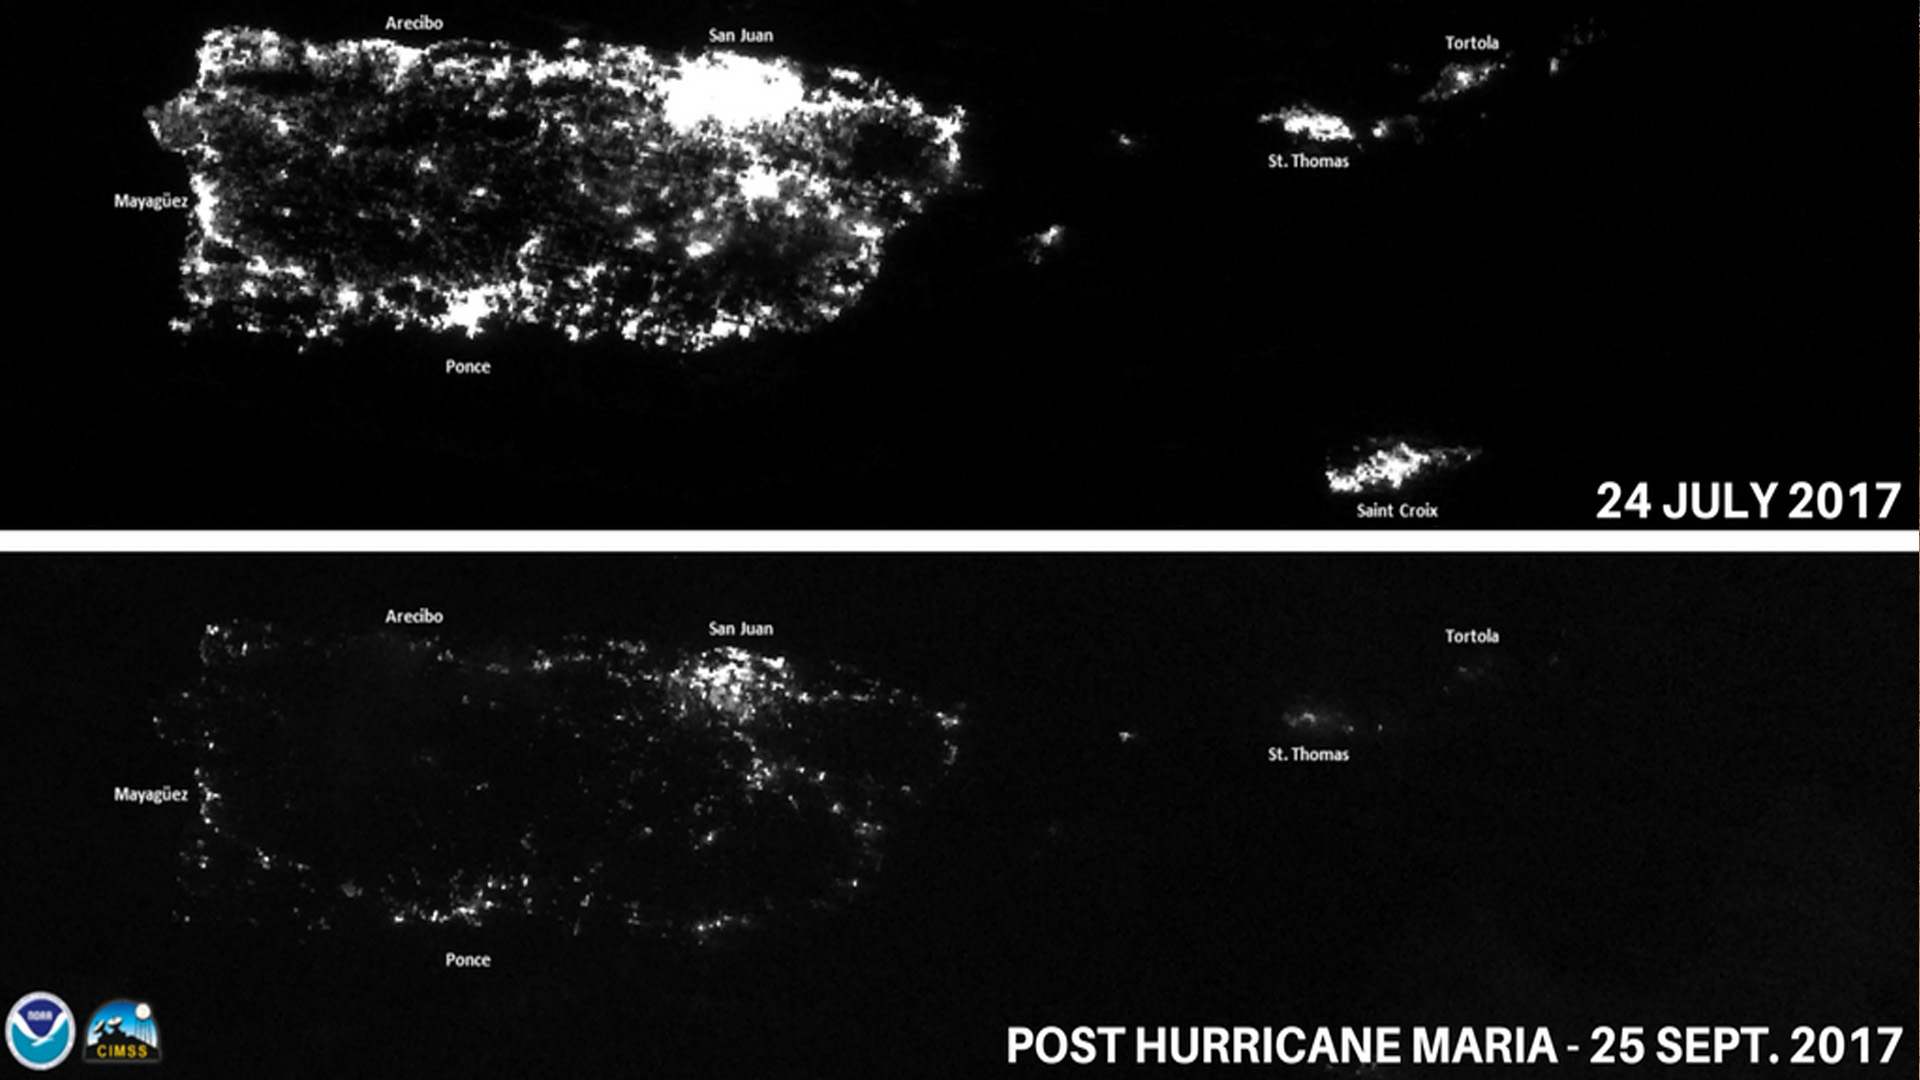
\includegraphics[width=0.75\textwidth]{after_hurricane.jpg}
    \caption{Comparison of lights at night in Puerto Rico before (top) and after (bottom) Hurricane Maria \cite{after_hurricane}}
    \label{fig:hurricane}
\end{figure}

\subsection{Problem Statement}
Our group has been tasked with designing a transportable disaster response system to assist HELP, Inc., a non-governmental organization, in providing relief for Puerto Rico after the hurricane. HELP, Inc. has provided us with information about potential candidate drones, cargo bay dimensions, medical package configurations, and anticipated medical package demand at five hospitals at the north and northeast parts of the island. Our goal is to derive the most efficient system of delivery routes and cargo container positioning which will allow us to:
\begin{enumerate}
    \item Deliver the required medical packages to each hospital on time, and 
    \item Conduct video reconnaissance of road networks.
\end{enumerate}

Figure \ref{fig:labeled_map} shows a section of the map of Puerto Rico where the locations that we are interested in have been labeled, along with the Euclidean distances (km) between them. The anticipated medical package demand at each of the five locations are specified in Table \ref{tab:package_demand}.

\begin{figure}[h]
    \centering
    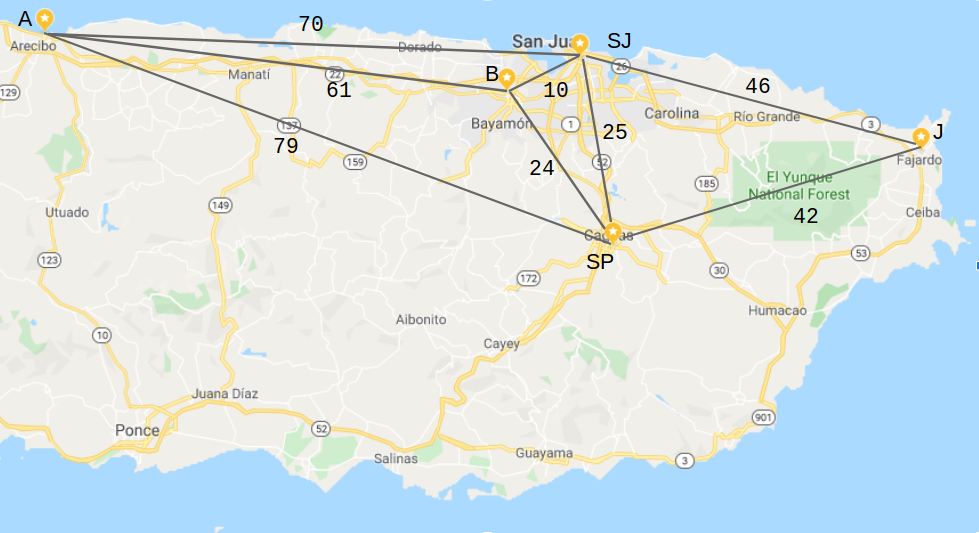
\includegraphics[width=0.75\textwidth]{map.png}
    \caption{Map of Puerto Rico with Locations of Interest (km)}
    \label{fig:labeled_map}
\end{figure}

\begin{table}[h]
    \centering
    \begin{tabular}{c|c|c|c}
    \hline Hospital Location & Requirement & Quantity & Frequency \\
    \hline J (Fajardo) & MED 1 & 1 & Daily  \\
             & MED 3 & 1 & Daily \\
    \hline SP (San Pablo) & MED 1 & 2 & Daily \\
              & MED 3 & 1 & Daily \\
    \hline SJ (San Juan) & MED 1 & 1 & Daily \\
              & MED 2 & 1 & Daily \\
    \hline B (Bayamon) & MED 1 & 2 & Daily \\
             & MED 2 & 1 & Daily \\
             & MED 3 & 2 & Daily \\
    \hline A (Arecibo) & MED 1 & 1 & Daily
    \end{tabular}
    \caption{Anticipated Medical Package Demand}
    \label{tab:package_demand}
\end{table}

\subsection{Supplies Given}
We are provided with the following list of supplies from which we will choose and construct our disaster response system:
\begin{itemize}
    \item Three standard ISO cargo containers for shipping our supplies, each with interior dimensions: 19'3"L $\times$ 7'8"W $\times$ 7'10"H. Converting the units to inches gives us Table \ref{tab:cargo_container_config}.
    \item Three types of medical packages (MED 1, MED 2, and MED 3) with configurations specified in Table \ref{tab:med_config}.
    \item Eight potential candidate drones (A-H) to deliver the medical packages with configurations and performance capabilities specified in Table \ref{tab:drones_info}.
    \item Two types of drone cargo bays and their configurations (Table \ref{tab:cargo_bay_config}).
\end{itemize}

\begin{table}[h]
    \centering
    \begin{tabular}{c|c|c|c}
    \hline Length (in.) & Width(in.) & Height (in.) & Volume (in$^3$)\\
    \hline 231 & 92 & 94 & 1,997,688
    \end{tabular}
    \caption{Cargo Container Configuration}
    \label{tab:cargo_container_config}
\end{table}

\begin{table}[h]
    \centering
    \begin{tabular}{c|c|c|c}
    \hline Container Type & Weight (lbs.) & Dimensions (in.) & Volume (in$^3$)\\
    \hline MED 1 & 2 & 14 $\times$ 7 $\times$ 5 & 490  \\
    MED 2 & 2 & 5 $\times$ 8 $\times$ 5 & 200 \\
    MED 3 & 3 & 12 $\times$ 7 $\times$ 4 & 336
    \end{tabular}
    \caption{Medical Package Configurations}
    \label{tab:med_config}
\end{table}

\begin{table}[h]
    \centering
    \begin{tabular}{c|c|c|c|c|c|c}
    \hline Drone & Dimensions & Maximum Payload & Speed &  Max Flight & Video & Cargo\\
    Model & (in.) & Capability (lbs.) & (km/hr) & Time (min.) & Capable & Bay Type \\
    \hline
    A & 45 $\times$ 45 $\times$ 25 & 3.5 & 40 & 35 & Y & 1 \\
    B & 30 $\times$ 30 $\times$ 22 & 8 & 79 & 40 & Y & 1 \\
    C & 60 $\times$ 50 $\times$ 30 & 14 & 64 & 35 & Y & 2 \\
    D & 25 $\times$ 20 $\times$ 25 & 11 & 60 & 18 & Y & 1 \\
    E & 25 $\times$ 20 $\times$ 27 & 15 & 60 & 15 & Y & 2 \\
    F & 40 $\times$ 40 $\times$ 25 & 22 & 79 & 24 & N & 2 \\
    G & 32 $\times$ 32 $\times$ 17 & 20 & 64 & 16 & Y & 2 \\
    H & 65 $\times$ 75 $\times$ 41 & N/A & N/A & Indefinite & N & N/A \\
    \end{tabular}
    \caption{Drone Configurations}
    \label{tab:drones_info}
\end{table}

\begin{table}[h]
    \centering
    \begin{tabular}{c|c}
    \hline Cargo Bay Type & Dimensions (in.) \\
    \hline 1 & 8 $\times$ 10 $\times$ 14 \\
    2 & 24 $\times$ 20 $\times$ 20
    \end{tabular}
    \caption{Cargo Bay Configurations}
    \label{tab:cargo_bay_config}
\end{table}

